
As was discussed in \sec\ref{sec:theory_www_production}, there are other decay
channels of the $WWW$ process besides the fully-leptonic decay channel,
which was the focus of Chapter \ref{sec:www}.  
In fact, one other decay channel for this process has been studied within 
ATLAS. This is the semi-leptonic channel where \wwwlljj. The details of this 
analysis are beyond the scope of this thesis. We can use the results of this channel,
however, along with those for the fully-leptonic decay channel, to obtain a stronger measurement
on the overall SM $WWW$ total cross-section measurement and limits on the aQGC signal reported than
those reported for just the fully-leptonic 
channel in \sec\ref{sec:measurement} and \sec\ref{sec:aqgc_limit}. 


In this chapter we will first summarize the results of the semi-leptonic study. 
This will be followed by a statistical combination of the fully-leptonic and semi-leptonic
results leading to an improved  
measurement on the SM $WWW$ total cross-section and limits on the 
aQGC signal.




\section{Search for \wwwlljj}
\label{sec:semilep}

%Mention that using same generator for signal, 
%same systematics, some differences in background estimation

%total cross-sections

%list selection

%fiducial cross-sections

%event yields

%c-factors

table of fiducial and cfactors

\section{Combined Cross-section Measurement}
\label{sec:combined_measurement}

The combined cross-section measurement is performed to 
measure the total cross-section of the $WWW$ process. 
The same expectation, likelihood, and profile likelihood
ratios in \eqn\eqref{eq:poisson_expectation},
\eqn\eqref{eq:poisson_likelihood}, and
\eqn\eqref{eq:profile_likelihood_ratio}, respectively.
The same methodology for extracting the measured fiducial
cross-section from
\sec\ref{sec:measurement} is used for extracting the combined
cross-section measurement except that the semi-leptonic channel
inputs are included along with the fully-leptonic channel
and that the measurement is extrapolated to the total
cross-section.
For the fully-leptonic channel,
the fiducial cross-section and C-factor inputs 
are taken from \tab\ref{tab:inputs_3l}
while the semi-leptonic channel inputs are taken from 
\tab\ref{tab:inputs_2l2j}.
The combined measurement on the signal strength, $\mu$, is translated
into a measurement on the total cross-section using the relation
\begin{equation}
\sigma^{\textrm{Total}}_{\textrm{Observed}} = \frac{\mu}{A} \sum_{i\in \textrm{Channels}} \sigma^{\textrm{Fiducial}}_i
\label{eq:sigmatot}
\end{equation}
where $A$ is the total acceptance which is the sum of the 
acceptance in each channel, $A_i$:
\begin{equation}
A = \sum_i A_i
\end{equation}
where $A_i$ is computed as
\begin{equation}
A_i = \frac{ \sigma^{\textrm{Fiducial}}_i }{ \sigma^{\textrm{Total}}}
\end{equation}
Where again the $\sigma^{\textrm{Fiducial}}_i $ are simply the fiducial
cross-sections in each channel taken from
\tab\ref{tab:inputs_3l} and \tab\ref{tab:inputs_2l2j}
and $\sigma^{\textrm{Total}}$ is the expected total cross-section
in \eqn\eqref{eq:total_www_xsec}, reprinted here for convenience:
\begin{equation}
\sigma^{\textrm{Total}}_{\textrm{Theory}}= 241.47\pm0.13 ~(\textrm{Stat.}) ~^{+10.33}_{-6.08} ~(\textrm{PDF}) ~\pm 6.3 ~(\textrm{Scale}) ~\textrm{fb} %uncertainty?
\end{equation}
The acceptance values for both the semi-leptonic and fully-leptonic channels 
are summarized here in \tab\ref{tab:acceptance}.
The total acceptance is found to be $A = 2.547 \times 10^{-3} \pm 0.039 \times 10^{-3}$.


\begin{table}[ht!]
\centering
\begin{tabular}{|cc||c|}
\hline
%& Channel & Signal Efficiency, $\varepsilon_i$  & Acceptance ($\times 10^{-4}$), $A_i$\\
& Channel & $A_i$ ($\times 10^{-3}$)\\
%&         & $\varepsilon_i$    &  $A_i$ \\
\hline\hline
\multirow{3}{*}{Fully-leptonic} & 0 SFOS & $0.512 \pm .019$ \\
				& 1 SFOS & $0.567 \pm .020$ \\
                                & 2 SFOS & $0.202 \pm .012$ \\
\hline
\multirow{3}{*}{Semi-leptonic} & $ee$     & $0.209 \pm .011$\\
                               & $e\mu$   & $0.519 \pm .016$\\
                               & $\mu\mu$ & $0.538 \pm .016$\\
\hline
\end{tabular}

\caption{Acceptance values, $A_i$, derived separately for each signal region. 
The sum of all of the acceptance
in each bin is used to compute the overall acceptance, $A$. 
Only statistical uncertainties are shown.}
\label{tab:acceptance}
\end{table}


The distribution of $q_0$ is shown 
in Fig.~\ref{fig:stat_measurement_significance} for the combination.  
The observed null p-value 
is found to be 0.1657 ($0.971~\sigma$) with an 
expected of 0.152 ($1.026~\sigma$).

%this is with reduced systematics. what is the effect of adding or removing more?
%plot should be redone with a bigger range
\begin{figure}[ht!]
\centering
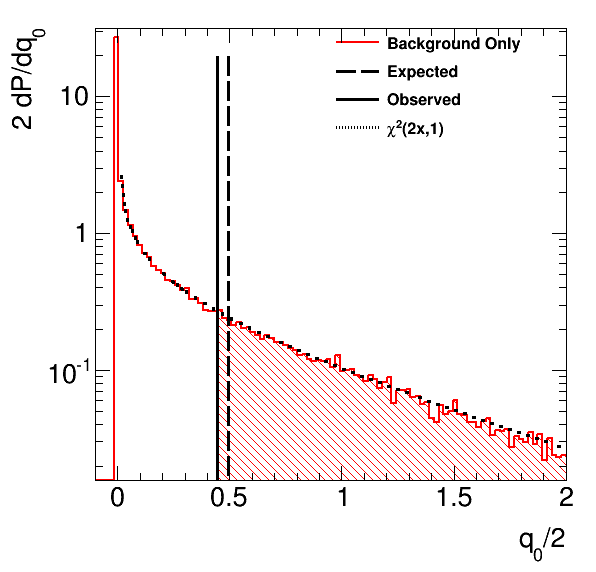
\includegraphics[width=0.70\columnwidth]{figures/combination/significance.png}
\caption{PDF of the background only hypothesis as a function of $q_0$ for the combination of all three channels. PDFs are determined 
using toy MC. The dashed black line represents the expected value of $q_0$ while the solid black line represents the observed value of $q_0$ seen in the data. The shaded area to the right
of this line represents the null p-value or the 
integral of the background hypothesis in the signal-like region.
The dotted black curve shows a $\chi^2$ distribution for 1 degree of freedom with which 
it can be seen is a good approximation of the 
the background only PDF.}
\label{fig:stat_measurement_significance}
\end{figure}

The negative log likelihood contour is shown
for the combination of all six channels in 
Fig.~\ref{fig:stat_measurement_interval_combination}.
The expected value and uncertainties for the fiducial cross-section is:
\begin{equation}
\sigma^{\textrm{Total}}_{\textrm{Expected}} = 241.47 ~ ^{+232}_{-199} \stat ~^{+152}_{-153}\syst ~\textrm{fb}
\end{equation}
while the observed fiducial cross-section is:
\begin{equation}
\sigma^{\textrm{Total}}_{\textrm{Observed}} = 227.03 ~ ^{+202}_{-198} \stat ~^{+154}_{-160} \syst ~\textrm{fb}
\end{equation}

\begin{figure}[ht!]
\centering
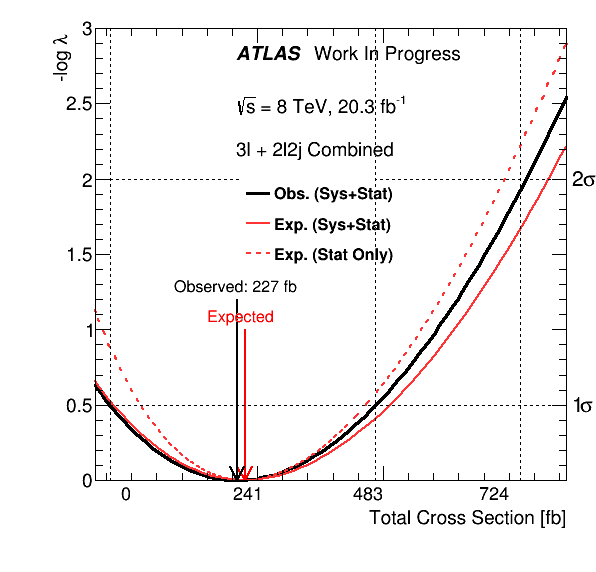
\includegraphics[scale=0.7]{figures/combination/interval_comb.png}
\caption{The profile likelihood contours evaluated as a function of the signal strength
for the combination of all three channels. 
The observed (black) and expected (red) contours are shown when considering only statistical uncertainty (dashed line) and when considering both statistical and systematic uncertainties (solid line).
The dotted black
lines pinpoint the location of the $1~\sigma$ and $2~\sigma$ total Gaussian uncertainties
on the measurement of the signal strength which corresponds to the minimum value of the contour.}
\label{fig:stat_measurement_interval_combination}
\end{figure}





%Acceptnace
%combined tables
%Measurement using same framework

\section{Combined aQGC Limits}
\label{sec:combined_aqgc}


\begin{table}[h!]
  \begin{center}
   \begin{tabular}{  |l| c | c c c | c c c | }
      \hline
      %&$\Lambda$& \multicolumn{6}{c|}{Expected Limit}  \\
      &$\Lambda$& \multicolumn{3}{c|}{Limits on F$_{s0}$ [$10^3~\TeV^{-4}$]}& \multicolumn{3}{c|}{Limits on F$_{s1}$ [$10^3~\TeV^{-4}$]}  \\
      &[\GeV]&  Lower & Upper & Measured & Lower & Upper & Measured  \\
      \hline
\multirow{5}{*}{Expected}      &500  & -8.12 & 8.92 & --- & -10.04 & 12.91 & --- \\ 
      &1000 & -3.7 & 4.16 & --- & -5.21 & 6.19 & --- \\ 
      &2000 & -2.35 & 2.57 & --- &-3.33 & 4.02 & --- \\ 
      &3000 & -1.87 & 2.24 & --- &-2.94 & 3.58 & --- \\ 
      &$\infty$ & -1.59 & 1.91 & --- & -2.54 & 3.09  & --- \\ 
      \hline \hline
\multirow{5}{*}{Observed}      &500  & -7.66 & 8.45 & 0.35  & -10.08 & 12.22 & 1.11 \\
      &1000 &  -3.11 & 3.87 & 0.40 & -4.77 & 5.81 & 0.85  \\
      &2000 &  -1.92 & 2.40 & 0.322  & -2.90 & 3.69 & 0.49 \\
      &3000 &  -1.6 & 2.09 & 0.37 & -2.48 & 3.18 & 0.47  \\
      &$\infty$& -1.27 & 1.76 & 0.34 & -2.10 & 2.71  & 0.40\\ 
      \hline
\end{tabular}


    \caption{Expected and observed limits on the aQGC Parameters.}
    \label{tab:aqgc_combined_1d}

  \end{center}
\end{table}


Combined limits on the aQGC signal use the same methodology
as in \sec\ref{sec:aqgc_limit} except that the inputs from the semi-leptonic
channel, described in \sec\ref{sec:semilep}, are included as well.
The resulting one-dimensional limits are listed in \tab\ref{tab:aqgc_combined_1d}
while the two-dimensional limts are shown in \fig\ref{fig:aqgc_combined_2d}.


\begin{figure}[h!]
\begin{center}

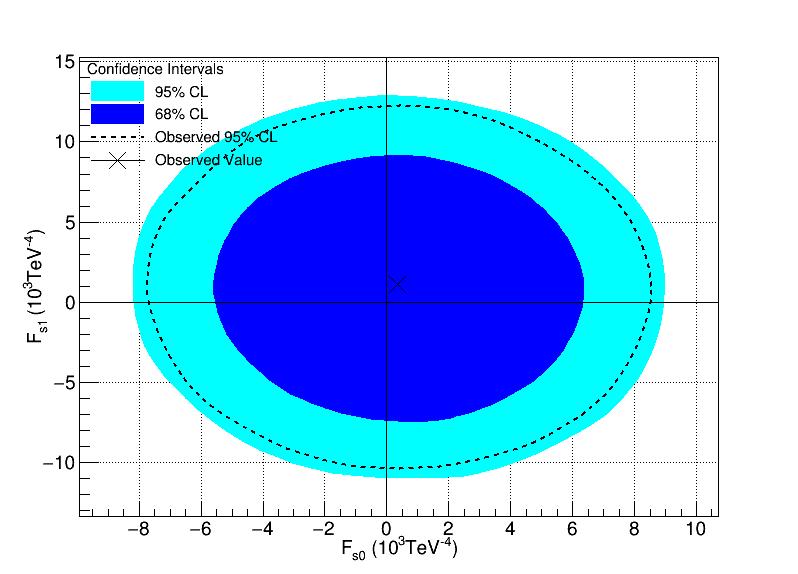
\includegraphics[width=0.45\textwidth]{figures/combination/Comb500-Lim.png}
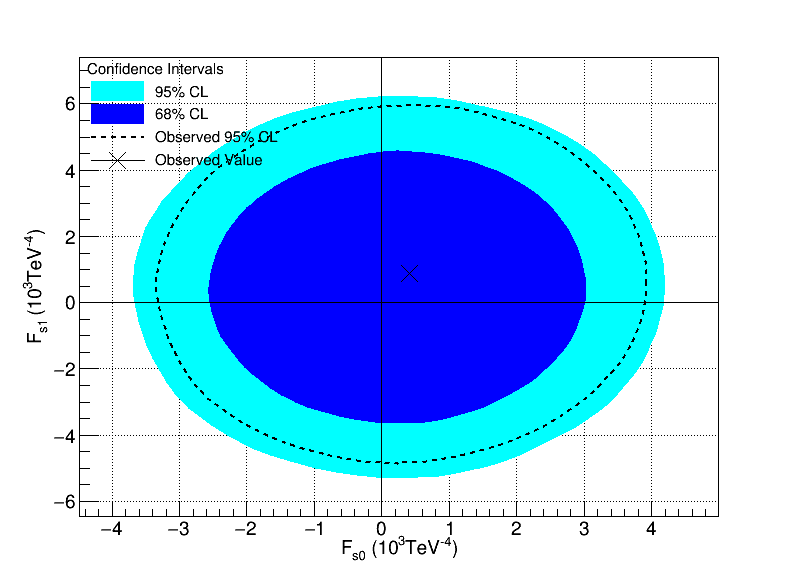
\includegraphics[width=0.45\textwidth]{figures/combination/Comb100-Lim.png}\\
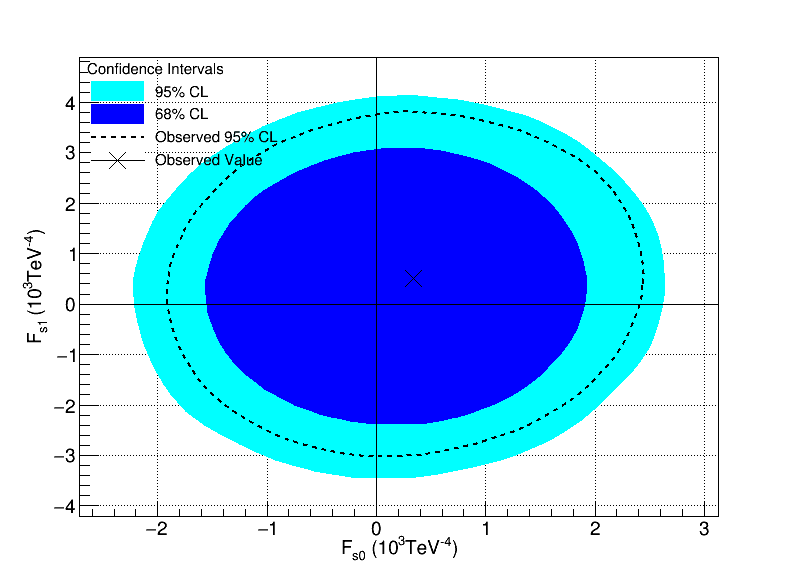
\includegraphics[width=0.45\textwidth]{figures/combination/Comb200-Lim.png}
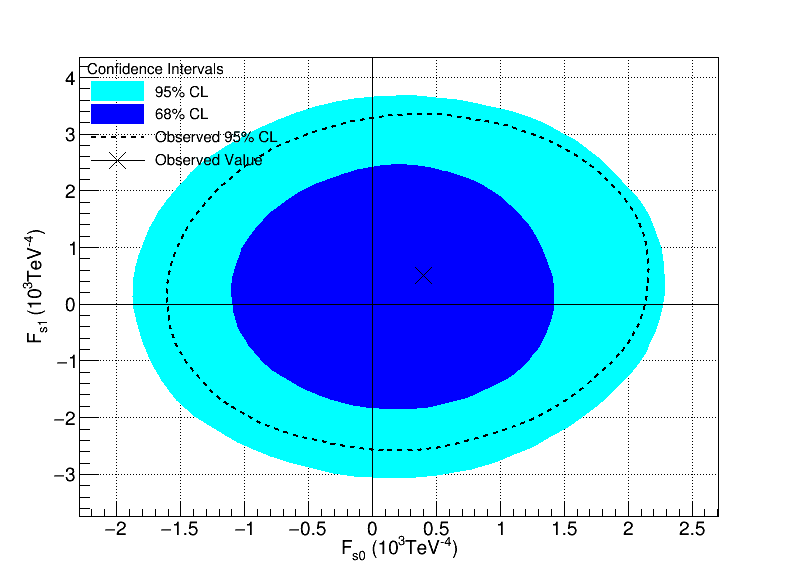
\includegraphics[width=0.45\textwidth]{figures/combination/Comb300-Lim.png}\\
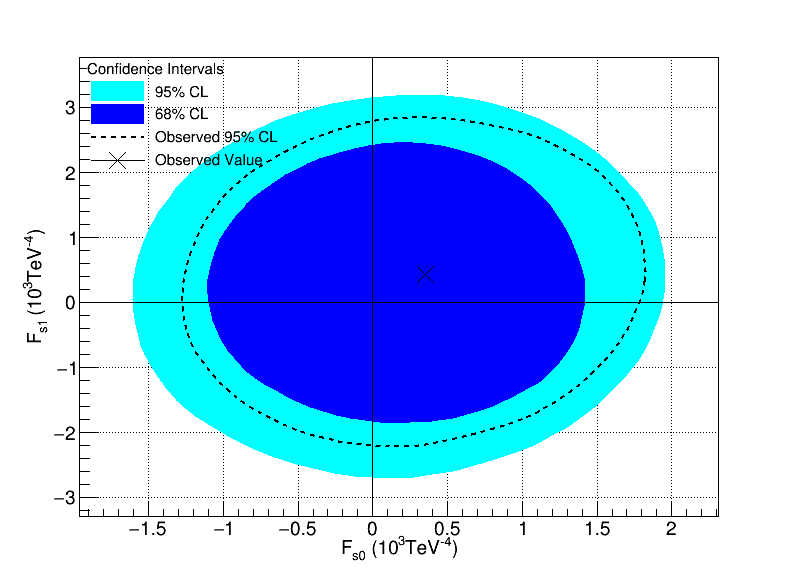
\includegraphics[width=0.45\textwidth]{figures/combination/CombUnit-Lim.png}
\end{center}
\caption{2D aQGC limits of Unitarized samples with scales 500,1000,2000,3000 and the Un-Unitarized Samples.(top left, top right, mid left, mid right, bottom)}
 \label{fig:aqgc_combined_2d}
 \end{figure}



